First start off simply by using cost complexity pruning where we tune the pruning paramater $\alpha$ by 10-fold cross-validation, which yields the tree in figure \ref{fig:DecisionTree} and a test accuracy of 82.9\%, which is lower than that of the most naive model, altough we again do conforim or hypothesis that $Rcyl$ and $vphi$ are important predictors.

Our tree-based models performed pretty similar, all with an accuracy that rounds to 87\%.

First we performed bagging using sklearns RandomForestClassifier and achieve a test accuracy of 86.8\%, where the predictors of highest importance $Rcyl$, $v\phi$ and $vRcyl$. We use this model to investigate our decision boundary in fig. \ref{fig:ratevsdb} and it seems that 0.5 is a really good threshold, since the sensitivity and precision curves cross at $T\approx0.5$. We also plot an ROC-curve in figure \ref{fig:ROC}, where the $AUC>0.5$ and our model is definitely better than chance.


\begin{figure}[h!]
    \centering
    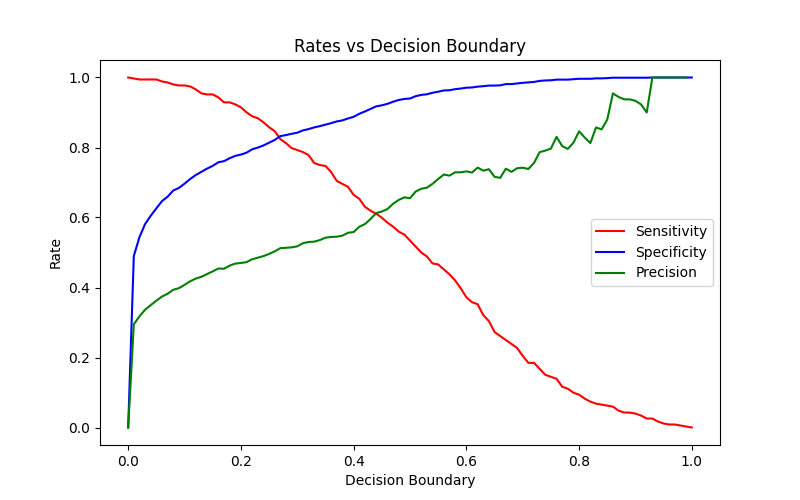
\includegraphics[width=0.75\columnwidth]{Plots/Rates_vs_DecisionBoundary.png}
    \caption{}
    \label{fig:ratevsdb}
\end{figure}

\begin{figure}[h!]
    \centering
    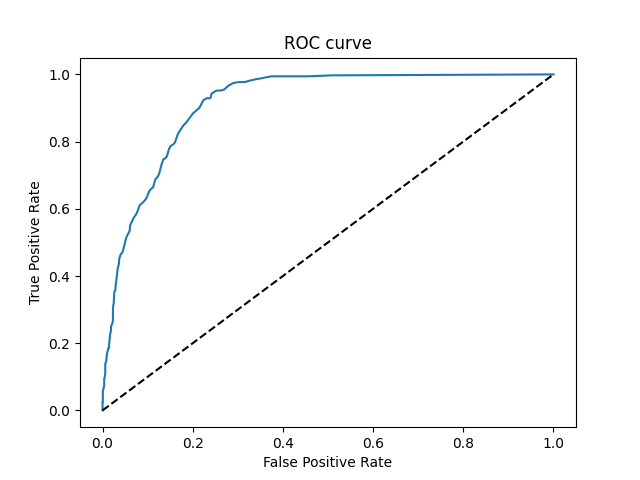
\includegraphics[width=0.8\columnwidth]{Plots/ROC_curve.png}
    \caption{}
    \label{fig:ROC}
\end{figure}
\newpage

We then perform random forrest for a range of maximum features in figure \ref{fig:randomforrest}. We noticed that our accuracy jumped quite a lot (within a small range), so we repeated the experiment for multiple random states, and the fluctuations seem to be due to random chance. The best performing models peak over 87\% and we cannot determine a best number of features, although it is probably more than 5.


\begin{figure}[h!]
    \centering
    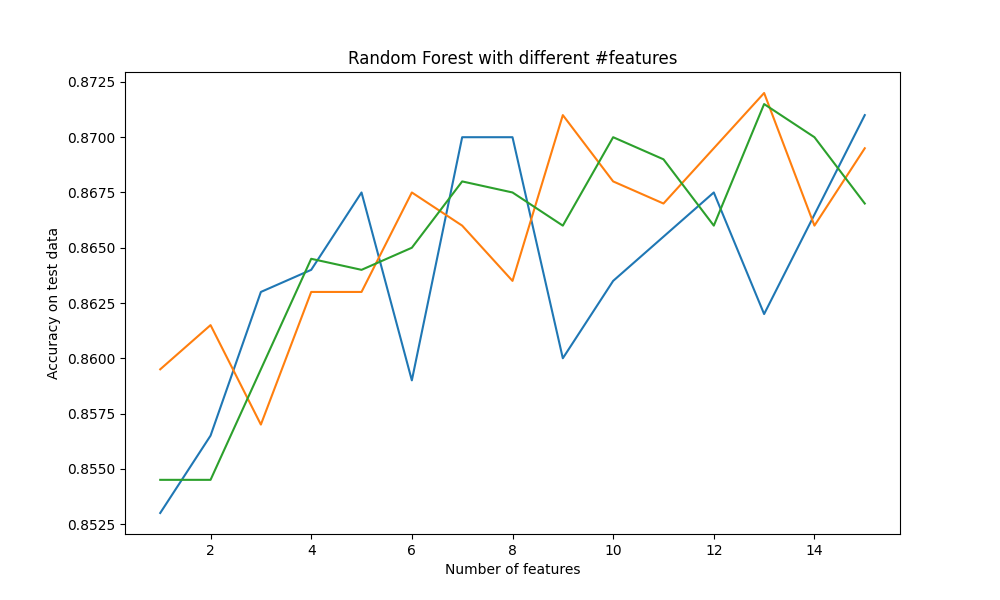
\includegraphics[width=0.75\columnwidth]{Plots/RandomForest.png}
    \caption{}
    \label{fig:randomforrest}
\end{figure}


At last we performed boosting. We trained 1000 trees with a maximum depth of 3 and variety shrinkage parameters $\lambda$, although the best performing one was with $\lambda = 0.01$, where we achieved a testing accuracy of 87.4\%. As seen in figure \ref{fig:accuracyvslambda} the accuracy shrinks for higher values of $\lambda$, which is just a sanity check, since the model is fine tuned more and more for smaller $\lambda$.


\begin{figure}[h!]
    \centering
    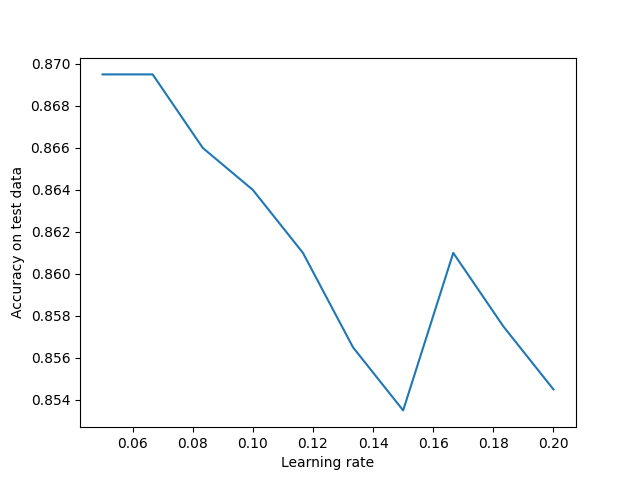
\includegraphics[width=0.75\columnwidth]{Plots/GradientBoosting.png}
    \caption{Gradient Boosting accuracy for different learning rates, $\lambda$}
    \label{fig:accuracyvslambda}
\end{figure}


In general the tree-based methods perform well compared to our other models, which is probable due to the fact that the trees are flexible enough to catch the small details, while keeping the variance down from taking the average.